\section{Lexikalische Elemente}
	\subsection{Sprachbeschreibung mit Grammatik \verweiscpp{3.1}}
	Die Grammatik einer Programmiersprache besteht (analog der Grammatik von nat�rlichen Sprachen) aus einer Menge von Regeln, die angibt, wie die einzelnen S�tze (Anweisungen), aus denen sich ein Programm zusammensetzt, aufgebaut sein m�ssen. Eine Regel besteht aus einem zu definierenden Symbol, gefolgt von einem Doppelpunkt und der Definition des Symbols. Alle Symbole einer Grammatik, die auf der linken Seite einer Regel (vor dem Doppelpunkt) erscheinen, werden als Non-Terminalsymbole bezeichnet. Symbole, die ausschliesslich auf der rechten Seite vorkommen, als Terminalsymbole. 
	
	\subsection{Bezeichner/Namen \verweiscpp{3.2}}
		\begin{minipage}[t]{5 cm}
		Bezeichner bezeichnen in einem C++ Programm:
		 	\begin{compactitem}
				\item Variablen
				\item Funktionen
				\item selbst definierte Datentypen
				\item Klassen
				\item Objekte \\...
		 	\end{compactitem}
	 	\end{minipage}
		 \hspace*{1.0cm}
		 \begin{minipage}[t]{5 cm}
		 Bezeichner k�nnen bestehen aus:
			\begin{compactitem}
				\item Buchstaben a-z, A-Z
				\item Ziffern 0-9
				\item Underscore \_
			\end{compactitem}
		\vspace*{0.2cm} 
		Das erste Zeichen eines Bezeichners darf keine Ziffer sein!
		\end{minipage}
		\hspace*{1.0cm}
		\begin{minipage}[t]{6 cm}
		Styleguide Variablen \& Funktionen:
			\begin{compactitem}
				\item mit Kleinbuchstaben beginnen	 			
				\item erster Buchstaben von zusammengesetzten W�rtern ist gross	
				\item keine Underscores
			\end{compactitem}
			\vspace*{0.2cm} 
			Beispiele: $counter$, $maxSpeed$, \\$getCount()$, $init()$, $setMaxSpeed()$	
		\end{minipage}	
	
	\subsection{Schl�sselw�rter \verweiscpp{3.3}}
	Schl�sselw�rter sind reservierte Bezeichner mit einer vorgegebenen Bedeutung und dienen zur Beschreibung von Aktionen und Objekten in C++ Programmen. Sie d�rfen daher nicht anderweitig verwendet werden.\\
	
		\begin{minipage}[c]{2.8cm}
			\begin{compactitem}
		 		\item $asm$
		 		\item $auto$				
		 		\item $bool$
		 		\item $break$
		 		\item $case$
		 		\item $catch$
		 		\item $char$
		 		\item $class$
		 		\item $const$
				\item $const\_cast$
		 	\end{compactitem}
	 	\end{minipage}
	 	\begin{minipage}[c]{3.2 cm}
		 	\begin{compactitem}	
		 		\item $continue$
		 		\item $default$
		 		\item $delete$
		 		\item $do$
		 		\item $double$
		 		\item $dynamic\_cast$
		 		\item $else$ 
		 		\item $enum$				
		 		\item $explicit$
		 		\item $extern$		 			
		 	\end{compactitem}
	 	\end{minipage}
	 	\begin{minipage}[c]{2.2 cm}
		 	\begin{compactitem}	
		 		\item $false$
		 		\item $float$
		 		\item $for$
		 		\item $friend$
		 		\item $goto$ 
		 		\item $if$				
		 		\item $inline$
		 		\item $int$
		 		\item $long$
		 		\item $mutable$		 			
		 	\end{compactitem}
	 	\end{minipage}
	 	\begin{minipage}[c]{3.6 cm}
		 	\begin{compactitem}	
		 		\item $namespace$
		 		\item $new$
		 		\item $operator$
		 		\item $private$				
		 		\item $protected$
		 		\item $public$
		 		\item $register$
		 		\item $reinterpret\_cast$
		 		\item $return$
		 		\item $short$		 		 	
		 	\end{compactitem}
	 	\end{minipage}
	 	\begin{minipage}[c]{2.4 cm}
		 	\begin{compactitem}	 
		 		\item $signed$
		 		\item $sizeof$				
		 		\item $static$
		 		\item $static_cast$
		 		\item $struct$
		 		\item $switch$
		 		\item $template$
		 		\item $this$
		 		\item $throw$
		 		\item $true$		 				 			
		 	\end{compactitem}
	 	\end{minipage}
	 	\begin{minipage}[c]{2.4 cm}
		 	\begin{compactitem}	
		 		\item $try$
		 		\item $typedef$
		 		\item $typeid$
		 		\item $typename$
		 		\item $union$
		 		\item $unsigned$
		 		\item $using$ 
		 		\item $virtual$				
		 		\item $void$
		 		\item $volatile$		 			
		 	\end{compactitem}
		\end{minipage}
	 	\begin{minipage}[c]{2.4 cm}
		 	\begin{compactitem}	
		 		\item $wchar\_t$
		 		\item $while$	
		 	\end{compactitem}
	 	\end{minipage}\\
	\subsection{Literale \verweiscpp{3.4}}
	Literale sind Zahlen, Wahrheitswerte oder Zeichenketten im Programmtext. So wie alle anderen Symbole eines Programms m�ssen auch sie nach bestimmten Regeln aufgebaut sein.
		\subsubsection{Ganze Zahlen}
		254 (dez), 035 (okt), 0x3f (hex), -34, 14L (long) 14U (unsigned), 14UL (unsigned long), ...
		\subsubsection{Fliesskommazahlen}
		254.89, -13.0, 3.45e23 (exp. Schreibweise), 4.65f (floar - Konstante), 3.14159L (long double), ...
		\subsubsection{Zeichen}
		Ein Zeichen-Literal wird in einfache Hochkommas eingeschlossen angegeben. Zeichen-Literale umfassen neben den druckbaren Zeichen auch Steuerzeichen. Um diese (nicht druckbaren) Zeichen darzustellen, wird eine sogenannte Escape-Sequenz verwendet. Sie wird mit dem Zeichen \textbackslash \ eingeleitet und bestimmt ein Zeichen aus dem ASCII mittels einer oktalen oder hexadezimalen Zahl. Um das Zeichen \textbackslash \ selbst darzustellen, wird \textbackslash\textbackslash \ verwendet. \\\\ 'A', '\textbackslash'' (einfaches Hochkomma), '\textbackslash \textbackslash' (Backslash), '\textbackslash b' (Backspace),'\textbackslash n' (Neue Zeile), '\textbackslash t' (Tabulator), '\textbackslash v' (Vertikaltabulator), '\textbackslash xFE' (Zeichen mit ASCII-Wert 18), ...
	
		\subsubsection{Zeichenketten}
		\begin{minipage}[t]{9 cm}
			Ein Zeichenketten-Literal ist eine (m�glicherweise auch leere) Sequenz von Zeichen, die in doppelten Hochkommas eingeschlossen ist. \\\\ "Hallo", "' "' (leere Zeichenkette), "Ha \textbackslash x41" (Ha A), ...
		\end{minipage}
		\hspace*{1cm}
		\begin{minipage}[t]{9 cm}
 			Beispiel $"'Ritchie"'$\\
 			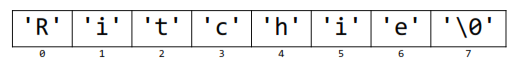
\includegraphics[width=0.6\textwidth]{pics/Zeichenkonstante.png}
 		\end{minipage}		
	\subsection{Operatoren und Begrenzer \verweiscpp{3.5}}
	Operatoren und Begrenzer sind einzelne Sonderzeichen bzw. Sequenzen von Sonderzeichen oder reservierten W�rter mit vordefinierter Bedeutung. Operatoren bestimmen Aktionen, die auf Programmobjekte ausgef�hrt werden k�nnen. Begrenzer wiederum trennen Symbole des Programmtexts voneinander.
	
	\subsection{Kommentare}
	Kommentare sind Anmerkungen im Programmtext, die f�r den Leser bestimmt sind. Der Compiler ignoriert sie und entfernt sie vor dem �bersetzen des Programms in Maschinencode aus dem Quelltext.\\\\
	// \ \ \ \ \ \ Einzeilige Kommentare \\
	/* */ \ \ Kommentare �ber mehrere Zeilen
	